\documentclass[border=4pt]{standalone}
\usepackage{tikz}
\begin{document}

\noindent
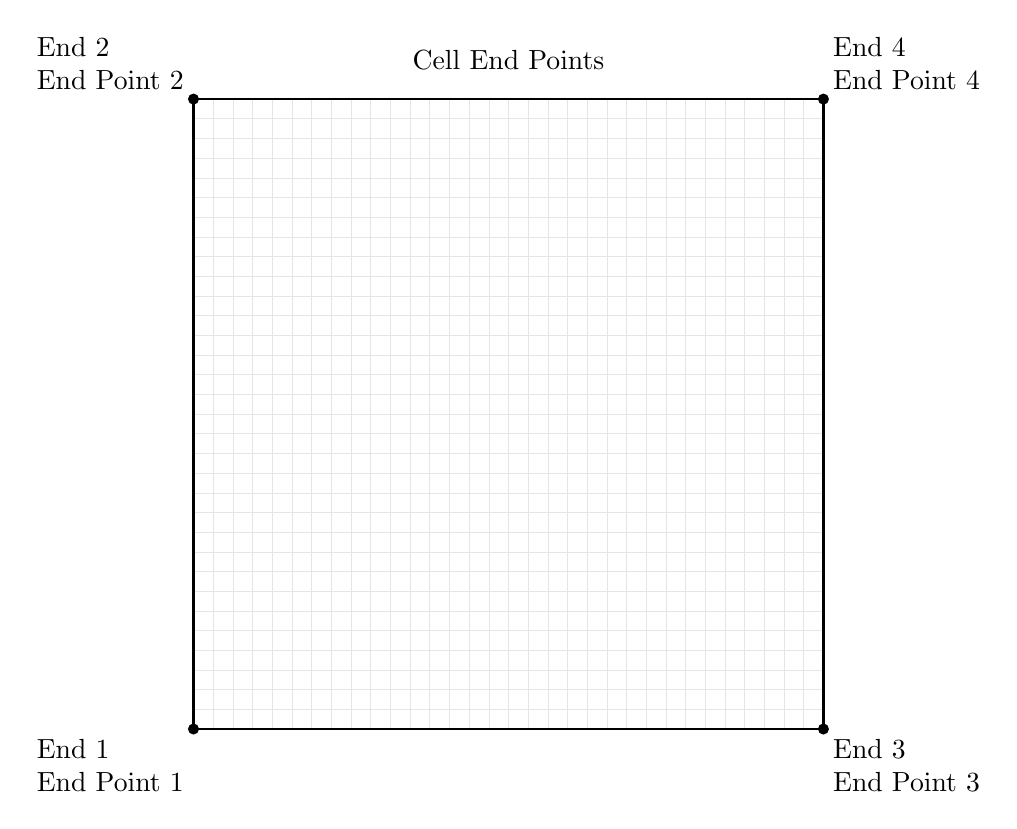
\begin{tikzpicture}[x=0.25cm,y=0.25cm,text centered]
  \draw[step=1,black!10,very thin] (0.0,0.0) grid (32.0,32.0);

  \node (TOPL) at (16,33) [above,align=center]  {Cell End Points};

  \draw[thick] (0,0) rectangle (32,32);

  \fill (0,0) circle(2pt);
  \node (0000) at (0,0) [below left,align=left]  {End 1\\End Point 1};
  \fill (0,32) circle(2pt);
  \node (0032) at (0,32) [above left,align=left]  {End 2\\End Point 2};
  \fill (32,0) circle(2pt);
  \node (3200) at (32,0) [below right,align=left]  {End 3\\End Point 3};
  \fill (32,32) circle(2pt);
  \node (3232) at (32,32) [above right,align=left]  {End 4\\End Point 4};

\end{tikzpicture}

\end{document}




